\section{Modelling}\label{capitolo2}
Al giorno d'oggi esistono una serie di computer il cui scopo principale non è quello di gestire informazioni, bensì quello di interagire con i sistemi fisici, questo tipo di computer è chiamato \emph{sistema embedded}, alcuni esempi di sistemi embedded sono:
\begin{itemize}
\item controlli automotive
\item avionica
\item dispositivi medici
\item controlli industriali
\item dispositivi di gestione e conservazione dell'energia
\end{itemize}
Un sistema embedded è un sistema di calcolo ma non principalmente un computer integrato con un insieme di processi fisici tramite sensori, attuatori ecc. il quale deve essere \emph{reattivo} ovvero deve rispettare dei vincoli temporali, è \emph{eterogeneo} in quanto formato da componenti hardware, software, componenti di rete; ed infine è \emph{distribuito} e \emph{concorrente}.
Un esempio di questo tipo di sistema lo troviamo sulle auto moderne dove sono presenti fino ad 80 computer denominate ECU (\emph{electronic control units}), esse variano dal controllo del motore e della trasmissione fino al controllo audio e di climatizzazione ma anche i display e la strumentazione di bordo. Sono presenti più di 100 milioni di linee di codice e tutti i sistemi sono collegati tramite CAN bus e oltre 2 km di cavi. Tale parte incide sempre più sul costo di una automobile.\\
Una parte molto importante di un sistema embedded è il software che viene eseguito su di esso in quanto deve sfruttare risorse limitate mantenendo performance elevate. Ad esempio la corretta esecuzione di un programma in \emph{C}, \emph{C\#}, Java etc. non tiene conto del tempo impiegato per l'esecuzione e ogni nostra astrazione è fondata su questa premessa; il tempo di esecuzione di un programma non è un fattore certo e ripetibile a meno che non prendiamo in considerazione una granularità molto grossa per l'analisi. Alcuni esempi che sfruttano l'irrilevanza del tempo nei sistemi normali sono il \emph{garbage collector}, la \emph{just-in-time} compilation, il \emph{power managment} e molti altri.\\
In un sistema embedded invece bisogna tener conto delle risorse limitate come la poca memoria e la dimensione della parola più corta e la frequenza di clock bassa. Per tener conto di queste limitazione ci si concentra sull'efficenza scrivendo software a basso livello (C, Assembly), si evitano sistemi operativi con molte funzionalità, si utilizzano architetture specializzate (DSP, Network) si utilizzano sistemi di interconnessione specializzati. Inoltre i sistemi embedded si differenziano da quelli \emph{general-purpose} in quanto devono rispettare dei vincoli temporali ("il più velocemente possibile" non è abbastanza), la concorrenza è intrinseca, le specifiche dei processori sono specializzate per rispettare i vincoli temporari supportare le operazioni più comuni e utilizzare specifici tipi di dati ed infine i programmi devono poter essere eseguiti \emph{per sempre} il reboot del sistema non è accettabile.\\
Il concetto di \emph{real-time} è più complicato del concetto del \emph{"prima possibile"}, in realtà esso indica dei limiti temporali che non possono essere valicati, oggi i programmatori di sistemi embedded costruiscono il sistema e successivamente lo testano per il timing. Un meccanismo basato sui modelli cerca di specificare il comportamento dinamico inclusi i vincoli temporari per poi \emph{"compilare"} un'implementazione che rispecchi le specifiche.\\
In molti casi i sistemi operativi real-time (\emph{RTOS}) sono utilizzati in maniere inappropriate, senza considerare particolari principi o funzionalità. Gli sviluppatori modificano le priorità fino a quando il prototipo non soddisfa i test. Tuttavia il sistema che ne risulta è fragile e un piccolo cambiamento nelle condizioni di operatività può causare grandi cambiamenti nel comportamento del sistema.\\
L'astrazione ha lo scopo di nascondere i dettagli dell'implementazione in modo da fornire una piattaforma sulla quale progettare. Un design basato su modelli può essere pensato a diversi livelli come strutturale, funzionale, orientato agli attori, ecc. questo permette uno sviluppo intuitivo del sistema tramite degli artifici che lo imitano. Un esempio è il \emph{modello matematico} il quale rappresenta il sistema tramite un insieme di definizioni e formule matematiche. Creare un modello matematico di tutte le parti di un sistema può portare alla costruzione automatica del sistema come avviene per un compilatore.\\
Esistono diverse tecniche di modello ognuna adatta a rappresentare un aspetto diverso del sistema, ad esempio:
\begin{itemize}
\item \textbf{Macchine a statti:} utile per rappresentare decisioni logiche sequenziali.
\item \textbf{Modelli basati sul flusso dei dati:} utili per esplorare il parallelismo e per il processo dei segnali.
\item \textbf{Modelli ad eventi discreti:} nel quale viene esplicitato il tempo.
\item \textbf{Modelli time-driven:} che studiano eventi periodici e azioni temporali
\end{itemize}
\subsection{Modelli di computazione}
Un \emph{modello di computazione} è un assegnamento di semantica, ovvero di significato, alla sintassi definita dal modello. Il \emph{MoC} definisce le regole per eseguire il modello, queste regole deteminano come gli attori intervengono sulla computazione, aggiornano i loro stati interni e interagiscono con l'esterno. Infine il modello di computazione definisce come diversi componenti comunicano tra loro.\\
Prendiamo in considerazione l'esempio di \figurename\,\ref{fig:parkschema} nel quale viene mostrato un contatore per le auto che entrano ed escono da un parcheggio.
\begin{figure}
\centering
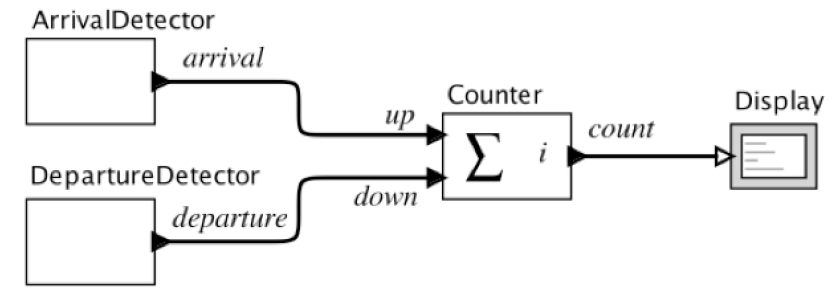
\includegraphics[scale=0.4]{img/parkschema.png}
\caption{Schema di un contatore per un parcheggio}\label{fig:parkschema}
\end{figure}
In questo caso vediamo che il sistema è composto da:
\begin{description}
\item[Segnali puri:] $up, \ down : \mathbb{R}\rightarrow\{absent,present\}$
\item[Attori discreti:]\emph{Contatore}:$(\mathbb{R}\rightarrow\{absent,present\})^P \rightarrow(\mathbb{R}\rightarrow\{absent\}\cup \mathbb{N})\_P=\{up,down\}$
\end{description}
Definiamo \emph{reazione} il fenomeno per cui per qualsiasi $t\in\mathbb{R}$ dove $up(t)\neq absent$ o  $down(t)\neq absent$ il \emph{Contatore} reagisce ovvero produce un output in $\mathbb{N}$ e modifica il suo stato interno.
Per ogni $t\in\mathbb{R}$ la porta \emph{p} ha una valorizzazione ovvero un assegnamento dei valori che per la porta $P=\{up,down\}$ corrisponde all'assegnamento sui due ingressi di uno dei due valori $\{absent, present\}$. Una reazione non è altro che una valorizzazione dell'output, in questo caso $count$ assume uno dei valori nel set $\{absent\}\cup \mathbb{N}$.\\
Un'altra definizione che dobbiamo dare è quella dello \emph{spazio degli stati} che non è altro che l'insieme degli stati in cui si può trovare il nostro contatore. Nel nostro caso il parcheggio ha un numero finito $M$ di posti disponibili perciò lo spazio degli stati per il nostro contatore è
$$State = \{0,1,2,3,\dots,M\}$$
Un modo per rappresentare il comportamento del nostro sistema è quello di utilizzare una \emph{Macchina a Stati Finiti}(\emph{FSM}) come quella di \figurename\,\ref{fig:parkfsm} nella quale possiamo distinguere alcuni tratti caratteristici:
\begin{description}
\item[Guardia:] insieme di valori che indicano i valori che devono essere presenti sugli input affinchè avvenga un cambio di stato, per l'arco che va da \emph{0} a \emph{1} la guardia è:
$$up \wedge \neg down $$ 
\item[Stato iniziale:] è quello indicato da una freccia entrante in questo caso è lo stato indicato da \emph{0}
\item[Valore di uscita:] è il valore che viene prodotto durante un passaggio di stato in questo caso è il valore del contattore, nella macchina a stati finiti è indicato dal valore a destra della \emph{guardia.}
\end{description}
\begin{figure}
\centering
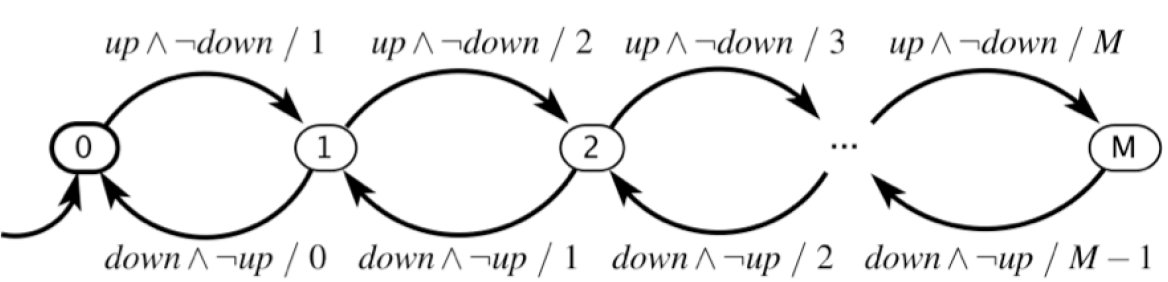
\includegraphics[scale=0.4]{img/parkfsm.png}
\caption{Macchina a stati finiti di un contatore per un parcheggio}\label{fig:parkfsm}
\end{figure}
Per definire una macchina a stati finiti formalmente sono necessari gli \emph{stati}, gli \emph{inputs}, gli \emph{outputs}, gli \emph{update} e lo \emph{stato iniziale}.\\
Una \emph{transizione di default} è una transizione che viene attivato solo quando le transizioni di default non sono attive e nessuna guardia è valutata come vera, un esempio di tale tipo di transizione è mostrata in \figurename\,\ref{fig:defaulttrans}.\\
\begin{figure}
\centering
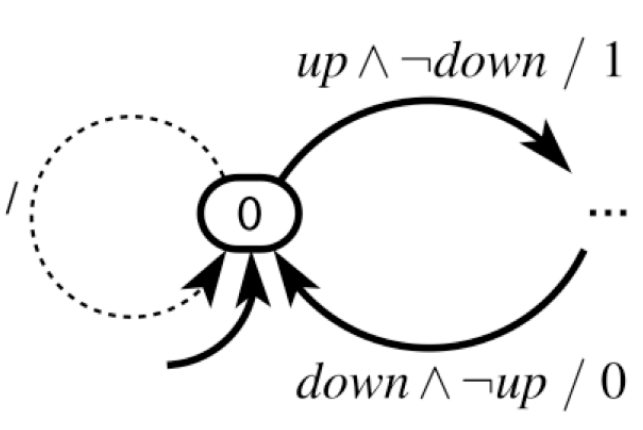
\includegraphics[scale=0.4]{img/defaulttrans.png}
\caption{Esempio di transizione di default}\label{fig:defaulttrans}
\end{figure}
Una transizione \emph{stuttering} è una tranzione di default implicita che viene abilitata in assenza di input e che non produce output. La \emph{ricettività} è una proprietà delle macchine a stati che afferma che per qualsiasi valore in input almeno una transizione è abilitata, le strutture con transizioni di default fanno in modo che le FSM siano ricettive.\\
Il \emph{determinismo} è una proprietà importante delle macchine a stati finite e afferma che in ogni stato per tutti i valori di input esattamente una transizione viene abilitata.\\
Il \emph{comportamento} di una FSM è definito come una sequenza di transizioni non \emph{stuttering}, una \emph{traccia} è un insieme di input, stati e output di un comportamento; un \emph{albero di computazione} è una rappresentazione grafica di tutte le possibile tracce. Tale proprietà fa si che le FSM siano analizzabili formalmente.\\
Il \emph{non determinismo} è la possibilità di avere, in una FSM, due possibili scelte per lo stesso valore di ingresso, un esempio di non determinismo è  mostrato in \figurename\,\ref{fig:nondetfsm}; la funzione di aggiornamento si trasforma in:
$$possibleUpdate : States \times Inputs \rightarrow 2^{States \times Outupts}$$
\begin{figure}
\centering
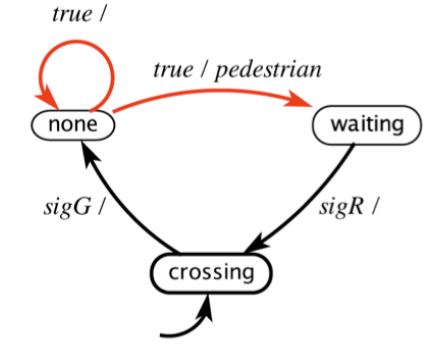
\includegraphics[scale=0.5]{img/nondetfsm.png}
\caption{Esempio di macchina a stati non deterministica}\label{fig:nondetfsm}
\end{figure}
Il non determinismo è molto utile nella fase di modellazione del sistema in quanto permette di modellizzare aspetti ignoti riguardante l'ambiente esterno, nascondere dettagli di una specifica, infine il non determinismo è più compatto da rappresentare.\\
Le macchine a stati finiti permettono di rappresentare un sistema in modo tale che esso sia analizzato matematicamente e manipolato, modellare l'ambiente attorno al sistema, modellare cosa il sistema deve o non deve fare ed infine è un modo per verificare se il sistema rispetta le specifiche.
\subsubsection{Composizione di macchine a stati}
Esistono tre tipi di composizione nelle macchine a stati e queste sono:
\begin{itemize}
\item Composizione side-by-side.
\item Composizione in cascata.
\item Composizione gerarchica.
\end{itemize}
Un esempio di composizione \emph{side-by-syde} è mostrata in \figurename\,\ref{fig:sidebyside}, in questo caso due stati sono posizionati in parallelo, la questione principale è come la macchina reagisce agli input, le possibilità sono due, i due stati reagiscono \emph{insieme} e allora si parla di composizione \emph{sincrona}; in caso in cui invece gli stati reagissero in maniera \emph{indipendente}, allora si parla di composizione \emph{asincrona}.
\begin{figure}
\centering
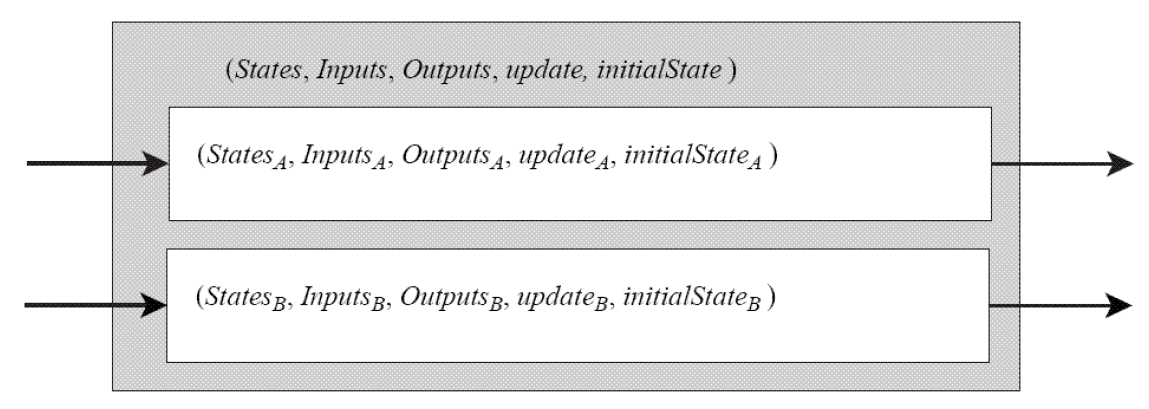
\includegraphics[scale=0.4]{img/sidebyside.png}
\caption{Esempio di composizione side-by-side}\label{fig:sidebyside}
\end{figure}
\paragraph{Composizione sincrona}
In questo caso gli stati reagiscono insieme, la macchina a stati che si ottiene è formata dalla composizione degli stati precedenti:
$$S_C=S_A \times S_B$$
La macchina a stati che si ottiene è mostrata in \figurename\,\ref{fig:sidesincrona} vediamo che due stati non sono raggiungibili in quanto non vi è alcun modo in cui gli ingressi possano arrivare a quel valore.
\begin{figure}
\centering
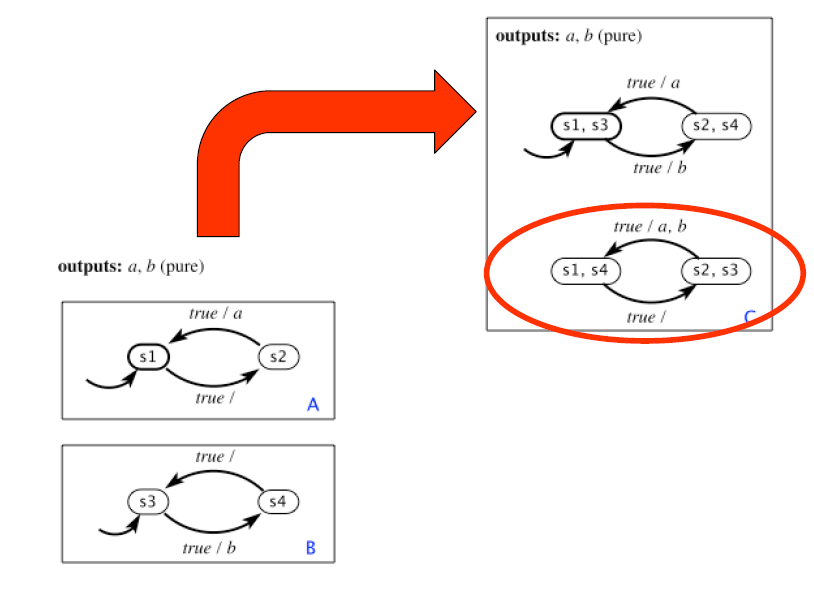
\includegraphics[scale=0.4]{img/sidesincrona.png}
\caption{Esempio di composizione side-by side sincrona}\label{fig:sidesincrona}
\end{figure}
Nel caso di composizione sincrona la nuova macchina che si viene a creare può essere espressa come:
$$
\begin{array}{lcl}
States & = & States_A \times States_B\\
Inputs & = & Inputs_A \times Inputs_B\\
Outputs & = & Outputs_A \times Outputs_B\\
initialState & = & initialState_A \times initialState_B\\
((S_A(n+1),S_B(n+1)),(o_A(n),o_B(n))) & = & update((S_A(n),S_B(n)),(i_A(n),i_B(n)))  
\end{array}
$$
dove 
$$
\begin{array}{rcl}
(S_A(n+1),o_A(n)) & = & update_A(S_A(n),i_A(n)) \mathtt{and} \\
(S_B(n+1),o_B(n)) & = & update_B(S_B(n),i_B(n)) 
\end{array}
$$
\paragraph{Composizione asincrona}
In questo caso gli stati reagiscono indipendentemente gli uni dagli altri, in questo caso tutti gli stati risultano raggiungibili come si vede dalla \figurename\,\ref{fig:sideasincrona} la composizione degli stati è eseguita tramite la semantica intervallata ed è il risultato di 
$$S_D=S_A\times S_B$$
\begin{figure}
\centering
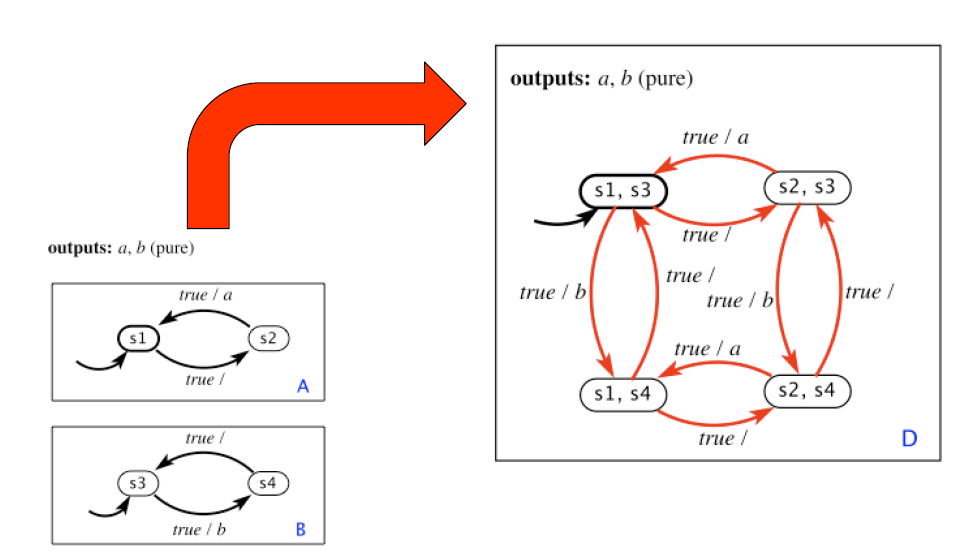
\includegraphics[scale=0.4]{img/sideasincrona.png}
\caption{Esempio di composizione side-by-side asincrona}\label{fig:sideasincrona}
\end{figure}
Nel caso invece di composizione asincrona la macchina a stati finita viene descritta da:
$$
\begin{array}{lcl}
States & = & States_A \times States_B\\
Inputs & = & Inputs_A \times Inputs_B\\
Outputs & = & Outputs_A \times Outputs_B\\
initialState & = & initialState_A \times initialState_B\\
((S_A(n+1),S_B(n+1)),(o_A(n),o_B(n))) & = & update((S_A(n),S_B(n)),(i_A(n),i_B(n)))  
\end{array}
$$
dove 
$$
\begin{array}{rcl}
(S_A(n+1),o_A(n)) & = & update_A(S_A(n),i_A(n)) \mathtt{and} S_B(n+1) = S_B(n) \& o_B = absent \mathtt{or}\\
(S_B(n+1),o_B(n)) & = & update_B(S_B(n),i_B(n)) \mathtt{and} S_A(n+1) = S_A(n) \& o_a = absent
\end{array}
$$
\subsubsection{Composizione in cascata}
La \emph{composizione in cascata} non è altro che il collegamento in serie di due macchine a stati come si vede dalla \figurename\,\ref{fig:cascade} dove l'output della prima macchina a stati è connesso all'input della seconda macchina. Anche in questo caso possiamo parlare di composizione sincrona e asincrona. 
\begin{figure}
\centering
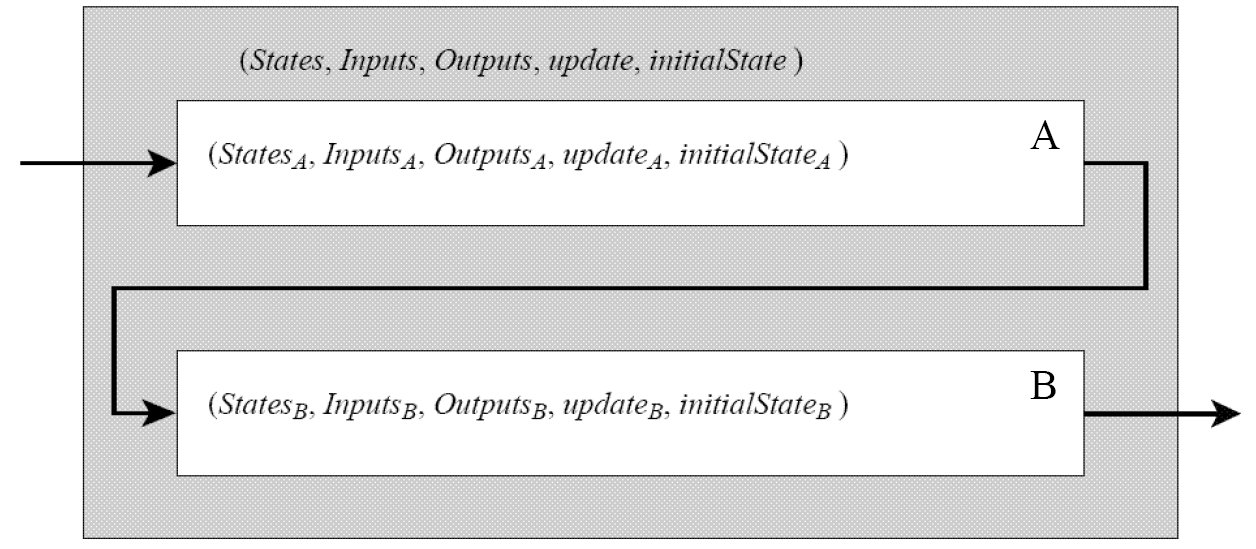
\includegraphics[scale=0.4]{img/cascade.png}
\caption{Esempio di composizione a cascata}\label{fig:cascade}
\end{figure}
Analizziamo ora un esempio di un semaforo nel quale una macchina a stati descrive il comportamento del semaforo utilizzato per le automobili \figurename\,\ref{fig:semaforoauto} mentre una seconda macchina a stati descrive il comportamento del semaforo pedonale \figurename\,\ref{fig:semaforoped}. 
\begin{figure}
\centering
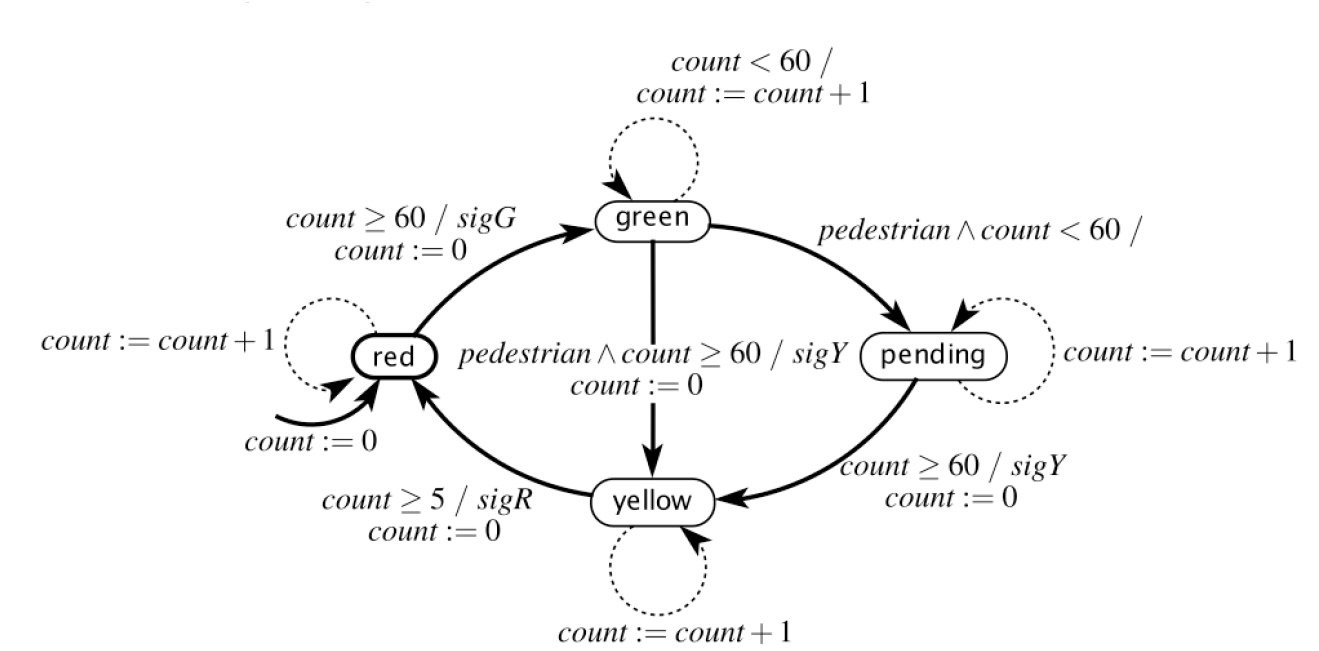
\includegraphics[scale=0.4]{img/semaforoauto.png}
\caption{FSM che modella il comportamento di un semaforo per le auto}\label{fig:semaforoauto}
\end{figure}
\begin{figure}
\centering
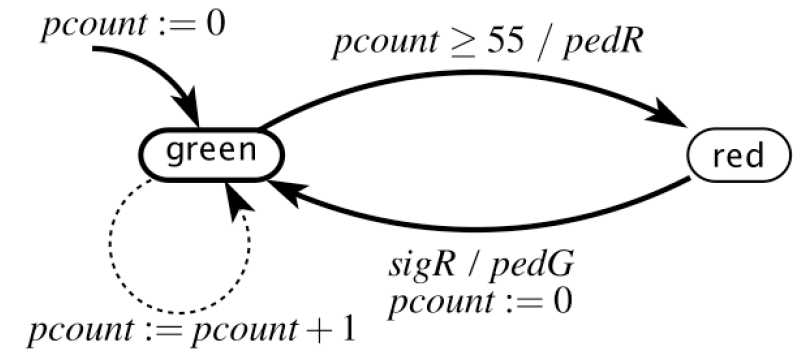
\includegraphics[scale=0.4]{img/semaforoped.png}
\caption{FSM che modella il comportamento di un semaforo per un attraversamento pedonale}\label{fig:semaforoped}
\end{figure}
In \figurename\,\ref{fig:semaforocomp} vediamo la composizione delle due macchine a stati finiti nella quale però sono stati rimossi gli stati non raggiungibili. In caso di composizione \emph{sincrona} la macchina reagisce simultaneamente nonostante sembra che esista una relazione causale tra le due. Ad esempio in questo caso sembrerebbe che la macchina agisca in modo sequenziale passando dal rosso al verde e viceversa ma bisogna tenere conto che in realtà gli stati che vengono raggiunti sono un insieme di stati e non vi è mai uno stato nel quale le due macchine non agiscono insieme.\\
\begin{figure}
\centering
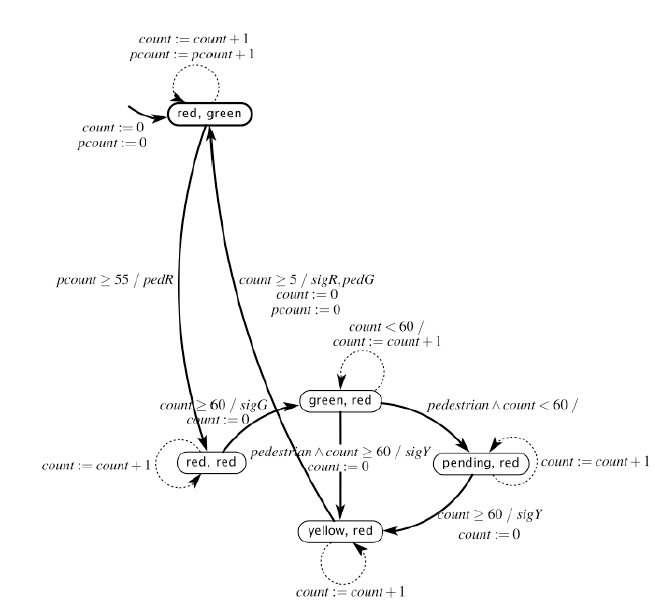
\includegraphics[scale=0.6]{img/semaforocomp.png}
\caption{Composizione in cascata delle due FSM precedenti}\label{fig:semaforocomp}
\end{figure}
Nel caso di composizione \emph{asincrona} invece le uscite di una macchina entrano negli ingressi dell'altra in modo indipendente dai cambiamenti delle macchine. Un esempio di composizione asincrona è mostrata in \figurename\,\ref{fig:cascadeasincrona}.\\
\begin{figure}
\centering
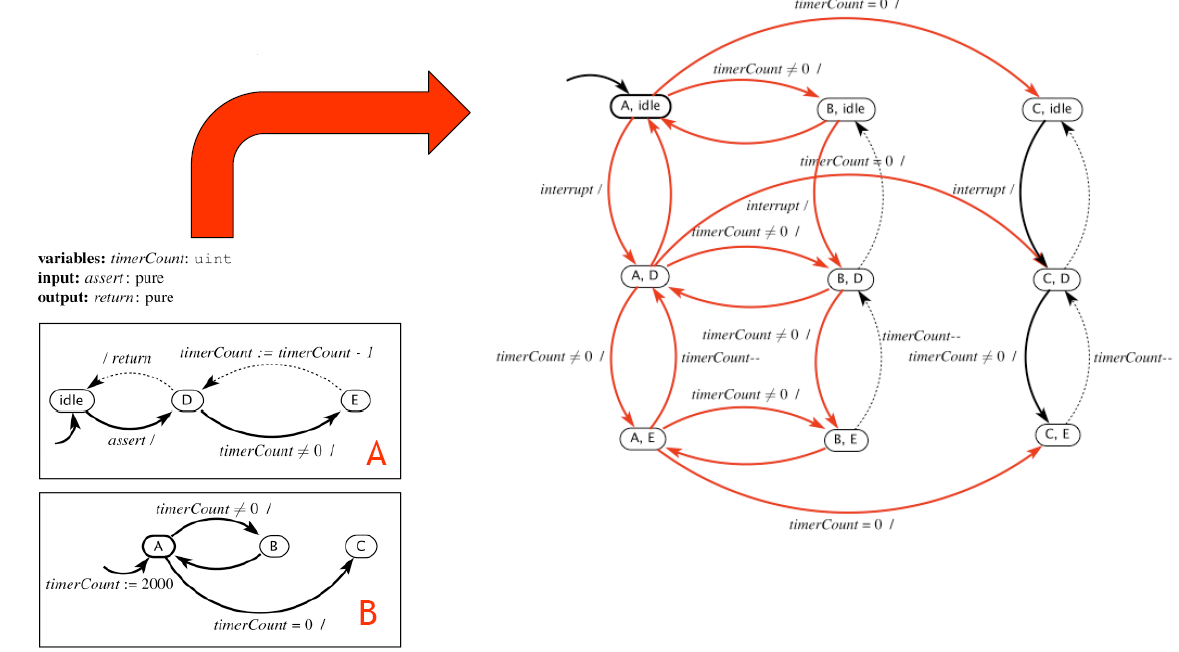
\includegraphics[scale=0.4]{img/cascadeasincrona.png}
\caption{Esempio di composizione in cascata asincrona}\label{fig:cascadeasincrona}
\end{figure}
\subsubsection{Composizione gerarchica}
Quando parliamo di composizione gerarchica facciamo riferimento ad un particolare tipo di FSM nella quale uno stato è rappresentato da una seconda FSM come nel caso di \figurename\,\ref{fig:gerarchica} in questo caso prima si raggiunge lo stato superiore e a quel punto si entra nello strato inferiore, nel caso entrambe le macchine producano un output questo non deve essere conflittuale.\\
\begin{figure}
\centering
\subfigure[]{
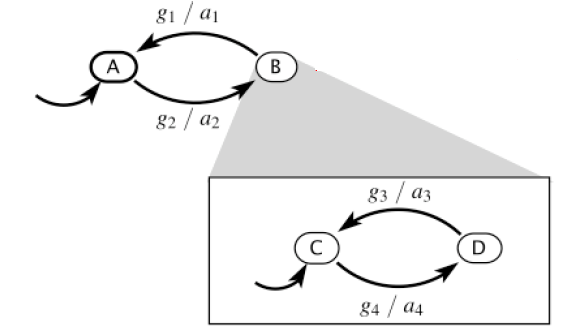
\includegraphics[scale=0.45]{img/gerarchia.png}
}
\subfigure[]{
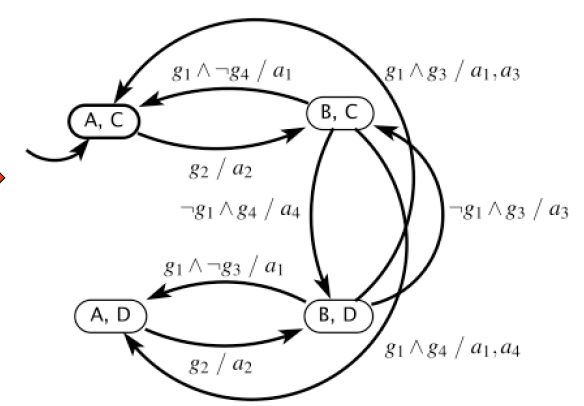
\includegraphics[scale=0.45]{img/gerarchiafsm.png}
}
\caption{Esempio di FSM gerarchica}\label{fig:gerarchica}
\end{figure}
A differenza degli altri casi il caso gerarchico permette diversi tipi di composizione. Ad esempio nel primo caso che analizziamo parliamo di \emph{memoria della transizione} ad esempio nella nostra macchina a stati quando raggiungiamo lo stato \emph{B} entriamo nella FSM composta dagli stati \emph{C} e \emph{D} a quel punto potremmo muoverci all'interno di quegli stati fino a quando non si presenti in ingresso il valore $g_1$ che ci fa tornare allo stato \emph{A}, nel caso di FSM con memoria una volta che torneremo nello stato \emph{B} ripartiremo dall'ultimo stato in cui abbiamo lasciato la macchina, un esempio delle transizioni è mostrato di seguito
$$A\xrightarrow{g_2/a_2}C\xrightarrow{g_4/a_4}D\xrightarrow{g_1/a_1}A\xrightarrow{g_2/a_2}D\xrightarrow{g_3\wedge g_1/a_3,a_1}A\dots$$
Esistono poi le FSM gerarchiche con rest come quella di \figurename\,\ref{fig:gerarchicareset} in questo caso la transizione che entra nello stato gerarchico è indicata da una freccia vuota. Il reset fa in modo che ad ogni ingresso in \emph{B} lo stato dal quale si parte sia sempre lo stato iniziale della sotto-FSM nel nostro esempio lo stato \emph{C}. Le transizioni in questo caso sono:
$$A\xrightarrow{g_2/a_2}C\xrightarrow{g_4/a_4}D\xrightarrow{g_1/a_1}A\xrightarrow{g_2/a_2}C\xrightarrow{g_4\wedge g_1/a_4,a_1}A\dots$$
\begin{figure}
\centering
\subfigure[]{
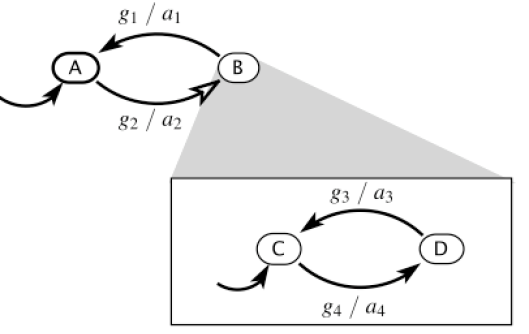
\includegraphics[scale=0.45]{img/gerarchiareset.png}
}
\subfigure[]{
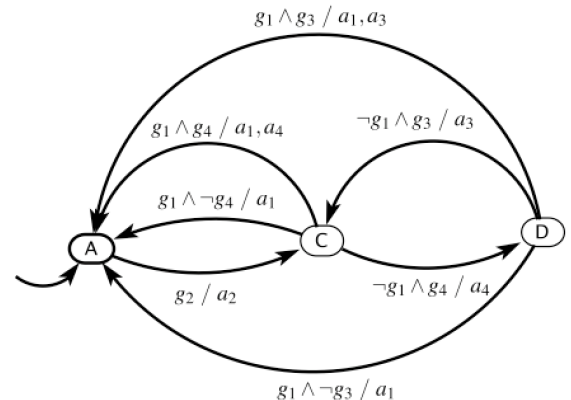
\includegraphics[scale=0.45]{img/gerarchiaresetfsm.png}
}
\caption{Esempio di FSM gerarchica con reset}\label{fig:gerarchicareset}
\end{figure}
L'ultima tipologia di composizione gerarchica è quella di \figurename\,\ref{fig:preemtiveger} ovvero una composizione gerarchica con \emph{preemtive}; il preemtive è un meccanismo per cui la valutazione della guardia che riporta la macchina nello stato \emph{A} è valutata prima di raggiungere lo stato corrente nella sottomacchina, nel caso la valutazione sia vera allora lo stato corrente non viene raggiunto.
\begin{figure}
\centering
\subfigure[]{
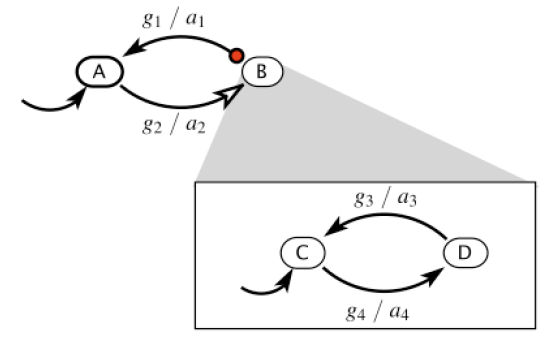
\includegraphics[scale=0.45]{img/preemtiveger.png}
}
\subfigure[]{
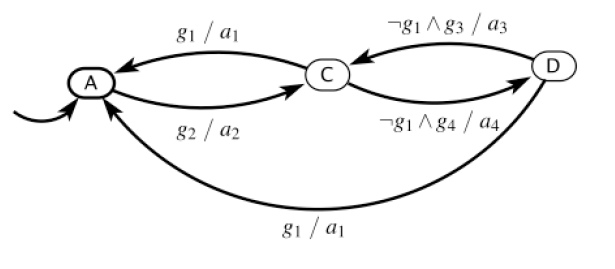
\includegraphics[scale=0.45]{img/preemtivegerfsm.png}
}
\caption{Esempio di FSM gerarchica con preemtive}\label{fig:preemtiveger}
\end{figure}
\subsection{Attori}
Gli attori non sono altro che dei componenti nei quali input e output sono esposti come in \figurename\,\ref{fig:attore} in questo caso però si tratta di modelli a tempo continuo, anche per gli  attori è possibile effettuare la composizione, la più comune è la composizione a \emph{feedback}.
\begin{figure}
\centering
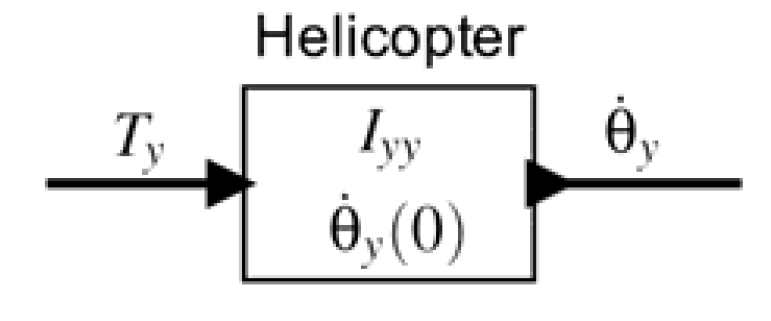
\includegraphics[scale=0.4]{img/attore.png}
\caption{Esempio di attore}\label{fig:attore}
\end{figure}
